\documentclass[border=6pt]{standalone}
\usepackage{lmodern}
\usepackage[T1]{fontenc}
\usepackage{amsmath}
\usepackage{xcolor}
\usepackage{tikz}
\usetikzlibrary{arrows.meta}
\definecolor{cgray}{HTML}{6E6C66}
\definecolor{cblue}{HTML}{2F7DC8}
\definecolor{camber}{HTML}{E0891E}
\definecolor{cred}{HTML}{C0392B}
\definecolor{cgreen}{HTML}{4E8E2A}
\definecolor{cink}{HTML}{2B2B2B}
\tikzset{>={Stealth[length=2.2mm]},crv/.style={line width=1.0pt,smooth,samples=120}}
% compatible scores (RCT controls AND compatible ECs) shifted to +b by shared model error;
% incompatible EC shifted further. sd ~0.8.
\newcommand{\gcomp}[1]{1.65*exp(0-((#1-2.0)*(#1-2.0))/1.28)}
\newcommand{\ginc}[1]{1.30*exp(0-((#1-4.6)*(#1-4.6))/1.28)}
\begin{document}
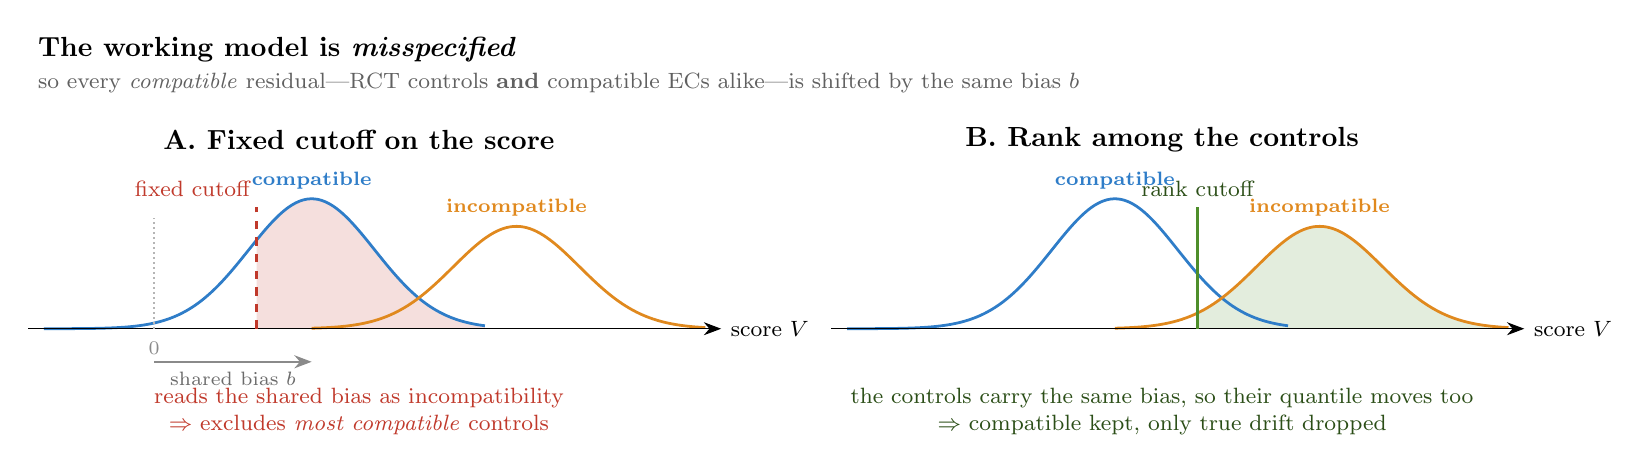
\begin{tikzpicture}[font=\small]

% ============ shared header ============
\node[font=\bfseries,anchor=west] at (-1.6,3.55) {The working model is \emph{misspecified}};
\node[font=\footnotesize,anchor=west,text=cink!75] at (-1.6,3.12)
  {so every \emph{compatible} residual---RCT controls \textbf{and} compatible ECs alike---is shifted by the same bias $b$};

% ============ Panel A: fixed cutoff ============
\begin{scope}
  \node[font=\bfseries] at (2.6,2.4) {A. Fixed cutoff on the score};
  % shade compatible mass beyond the fixed cutoff (false exclusions)
  \fill[cred!16] (1.3,0) -- plot[domain=1.3:4.2,samples=60] (\x,{\gcomp{\x}}) -- (4.2,0) -- cycle;
  \draw[cblue,crv] plot[domain=-1.4:4.2] (\x,{\gcomp{\x}});
  \draw[camber,crv] plot[domain=2.0:7.0] (\x,{\ginc{\x}});
  \draw[->] (-1.6,0) -- (7.2,0) node[right,font=\footnotesize]{score $V$};
  % correct-model center (0) and the shared bias arrow
  \draw[cink!35,densely dotted,line width=0.8pt] (0,0) -- (0,1.4);
  \node[cink!55,font=\scriptsize,below] at (0,-0.05) {$0$};
  \draw[->,cink!55,line width=0.8pt] (0,-0.42) -- node[below,font=\scriptsize,text=cink!70]{shared bias $b$} (2.0,-0.42);
  % fixed cutoff
  \draw[cred,dashed,line width=1.1pt] (1.3,0) -- (1.3,1.55);
  \node[cred,font=\footnotesize,anchor=south east] at (1.34,1.55) {fixed cutoff};
  \node[cblue,font=\scriptsize\bfseries,anchor=south] at (2.0,{\gcomp{2.0}}) {compatible};
  \node[camber,font=\scriptsize\bfseries,anchor=south] at (4.6,{\ginc{4.6}}) {incompatible};
  \node[cred,font=\footnotesize,align=center] at (2.6,-1.05)
     {reads the shared bias as incompatibility\\ $\Rightarrow$ excludes \emph{most compatible} controls};
\end{scope}

% ============ Panel B: rank ============
\begin{scope}[xshift=10.2cm]
  \node[font=\bfseries] at (2.6,2.4) {B. Rank among the controls};
  \fill[cgreen!16] (3.05,0) -- plot[domain=3.05:7.0,samples=60] (\x,{\ginc{\x}}) -- (7.0,0) -- cycle;
  \draw[cblue,crv] plot[domain=-1.4:4.2] (\x,{\gcomp{\x}});
  \draw[camber,crv] plot[domain=2.0:7.0] (\x,{\ginc{\x}});
  \draw[->] (-1.6,0) -- (7.2,0) node[right,font=\footnotesize]{score $V$};
  \draw[cgreen,line width=1.2pt] (3.05,0) -- (3.05,1.55);
  \node[cgreen!55!black,font=\footnotesize,anchor=south] at (3.05,1.55) {rank cutoff};
  \node[cblue,font=\scriptsize\bfseries,anchor=south] at (2.0,{\gcomp{2.0}}) {compatible};
  \node[camber,font=\scriptsize\bfseries,anchor=south] at (4.6,{\ginc{4.6}}) {incompatible};
  \node[cgreen!55!black,font=\footnotesize,align=center] at (2.6,-1.05)
     {the controls carry the same bias, so their quantile moves too\\ $\Rightarrow$ compatible kept, only true drift dropped};
\end{scope}

\end{tikzpicture}
\end{document}
